%%%%%%%%%%%%%%%%%%%%%%%%%%%%%%%%%%%%%%%%%%%%%%%%%%%%%%%%%%%%%%%%%%%%%%%%%%%%%%%%%%%%%%%%%%
%%
%% Description:		This is an example presentation using the beamerthemedhbw
%%
%%					The beamerthemedhbw is based on jacksbeamertheme
%%					(https://github.com/JacknJo/jacksbeamertheme)
%%
%% Author:			Hannes Bartle																				
%% 					DHBW Ravensburg Campus Friedrichshafen		
%%					September 2016	
%% 
%% The beamerthemedhbw is free software: you can redistribute it and/or modify
%% it under the terms of the GNU General Public License as published by
%% the Free Software Foundation, either version 3 of the License, or
%% (at your option) any later version.
%% 
%% The beamerthemedhbw is distributed in the hope that it will be useful,
%% but WITHOUT ANY WARRANTY; without even the implied warranty of
%% MERCHANTABILITY or FITNESS FOR A PARTICULAR PURPOSE.  See the
%% GNU General Public License for more details.
%% 
%% You should have received a copy of the GNU General Public License
%% along with the beamerthemedhbw.  If not, see <http://www.gnu.org/licenses/>.
%% 
%% 
%%%%%%%%%%%%%%%%%%%%%%%%%%%%%%%%%%%%%%%%%%%%%%%%%%%%%%%%%%%%%%%%%%%%%%%%%%%%%%%%%%%%%%%%%%


\documentclass[	12pt, 				
				t,					
				aspectratio=169,
				%handout-PLACEHOLDER
				]{beamer}

\usepackage{dhbwstyle}

\title{Collections, Iteratoren und Exceptions}

\begin{document}
	
	\begin{frame}[noframenumbering]
		\titlepage
	\end{frame}


	\begin{frame}{Inhalt}
		\tableofcontents
	\end{frame}
    
    \outlineFrame{Collections Framework}
    
    \outlineSubframe{Allgemeines}
\begin{frame}{Collections}{Was genau ist das eigentlich? (Vgl. \cite{collection1}}
    \begin{itemize}[<+->]
        \item Kann sowohl bezeichnen:
        \begin{itemize}
            \item Das Collections \textit{Framework}
            \item Das Collections \textit{Interface} (Als Teil des Collection Frameworks)
        \end{itemize}
        \item Collections sind grundlegend:
        \begin{itemize}
            \item Datenstrukturen um eine Gruppe von Elementen zu speichern...
            \item ...und zu manipulieren
        \end{itemize}
        \item Das Collections Framework ist eine Zusammenfassung aus Klassen, Interfaces und Algorithmen
    \end{itemize}
\end{frame}

\begin{frame}{Collections Framework}{Übersicht}
    \begin{figure}
    \centering
    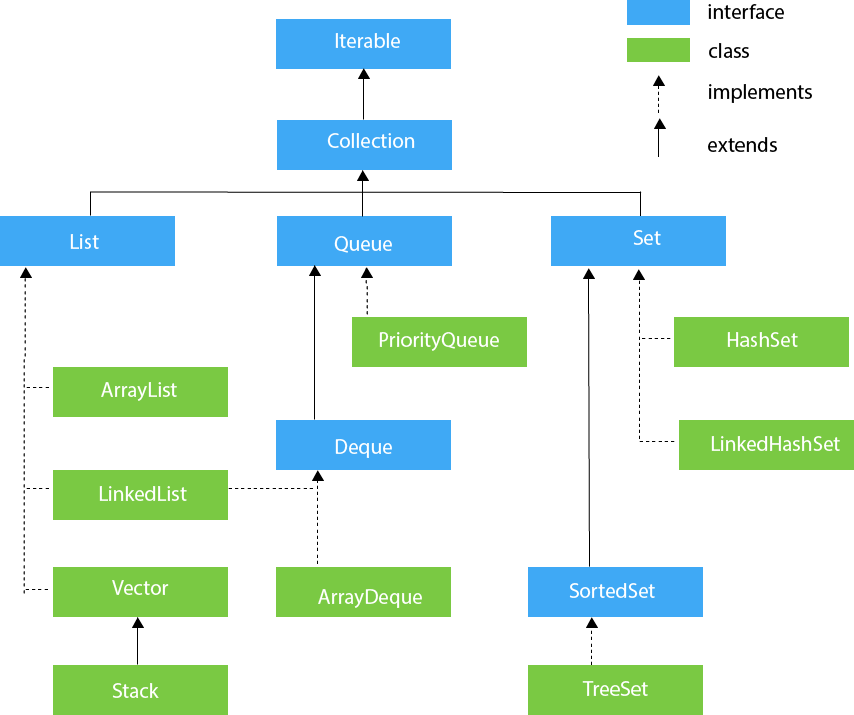
\includegraphics[height=5cm]{graph/java-collection-hierarchy}
    \caption{Quelle: \cite{collection1}}
    \end{figure}
\end{frame}

\begin{frame}{Collections Framework}{Übersicht}
    \begin{itemize}[<+->]
        \item Bestes Anwendungsbeispiel für Generics
        \begin{itemize}
            \item Listen sind für \textbf{alle} Klassen verwendbar...
            \item ...ohne, dass irgendwelche Änderungen vorgenommen werden müssen
        \end{itemize}
        \item C++ Äquivalent: STL Containers
        \begin{itemize}
            \item Seit C++11 teil des Standards
            \item Umfasst einige Datenstrukturen, die Collections nicht haben
        \end{itemize}
    \end{itemize}
\end{frame}

\outlineSubframe{Interfaces\&Klassen}
\begin{frame}{Collection}{Der Grundstein (Vgl. \cite{orac:collection}}
    \begin{itemize}[<+->]
        \item Grundlegendes Interface für alle Subinterfaces und Klassen
        \item Definiert grundlegende Methoden zum:
        \begin{itemize}
            \item Hinzufügen...
            \item Entfernen...
            \item Vergleichen...
            \item Zählen...
            \item ...von Elementen
        \end{itemize}
        \item Noch keine (direkte) Methode zum \textit{lesen} von Elementen
    \end{itemize}
\end{frame}

\begin{frame}{List}{}
    \begin{itemize}[<+->]
        \item Grundsätzliche Struktur für Listen von Elementen
        \item Keine Einschränkung der enthaltenen Elemente
        \item Erlaubt random access von Elementen
        \item Reihenfolge der Elemente wird beibehalten
        \begin{itemize}
            \item Heißt, Elemente liegen in der Reihenfolge vor, wie sie hinzugefügt wurden
            \item Sofern die Liste nicht anderweitig modifiziert wurde (Sortieren o.Ä.)
        \end{itemize}
    \end{itemize}
\end{frame}

\begin{frame}{ArrayList}{Implementierung des List Interfaces}
    \begin{itemize}[<+->]
        \item Daten werden in dynamsichen Array gespeichert
        \item Größe von diesem wird nach Bedarf (im Hintergrund oder auf Anfrage) angepasst
        \item Sehr ähnlich zur \texttt{Vector} Implementierung...
        \begin{itemize}
            \item Jedoch nicht synchronisiert...
            \item ...und deshalb nicht für multithreaded Anwendungen geeignet
        \end{itemize}
    \end{itemize}
\end{frame}

\begin{frame}{LinkedList}{Implementierung des List Interfaces}
    \begin{itemize}[<+->]
        \item Daten werden als Double-Linked-List gespeichert
        \item Ermöglicht Zugriff von beiden "`Enden"' der Liste
        \item Implementiert sowohl \texttt{List} Interface, als auch \texttt{Deque} Interface
        \item Ähnlich wie \texttt{ArrayList}: Nicht thread-safe
    \end{itemize}
\end{frame}

\begin{frame}{Vector}{}
    \begin{itemize}[<+->]
        \item Existierte schon vor dem \texttt{Collections} Framework
        \item Wurde in dieses aufgenommen
        \item Im Grunde ähnlich wie \texttt{ArrayList}
        \item Aber: Thread-Safe
    \end{itemize}
\end{frame}


\begin{frame}{Queue}
    \begin{itemize}[<+->]
        \item Repräsentiert eine "`Warteschlange"'
        \item Für Elemente gilt \textbf{FIFO}:
        \begin{itemize}
            \item \textbf{F}irst \textbf{I}n \textbf{F}irst \textbf{O}ut
            \item Nur Zugriff auf vorderstes Element
        \end{itemize}
        \item Reihenfolge der Elemente nicht unbedingt beibehalten
        \begin{itemize}
            \item \texttt{PriorityQueue} sortiert Element automatisch
        \end{itemize}
    \end{itemize}
\end{frame}

\begin{frame}{Deque}
    \begin{itemize}[<+->]
        \item \textbf{D}ouble \textbf{e}nded \textbf{Que}ue
        \item Subklasse von \texttt{Queue}
        \item Erlaubt jedoch Zugriff auf erstes und letztes Element der Liste
        \item Somit Verwendung auch zB. als \textbf{LIFO} Liste
        \begin{itemize}
            \item \textbf{L}ast \textbf{I}n \textbf{F}irst \textbf{O}ut
        \end{itemize}
    \end{itemize}
\end{frame}

\begin{frame}{Set}
    \begin{itemize}
        \item Vergleichbar mit einer mathematischen Menge
        \begin{itemize}
            \item Jedes Element kann genau einmal vorkommen
        \end{itemize}
        \item Je nach Implementierung...
        \begin{itemize}
            \item ...wird die Reihenfolge der Daten beibehalten
            \item ...werden die Daten strukturiert
        \end{itemize}
    \end{itemize}
\end{frame}

\begin{frame}{Map}{Die Collection die keine ist}
    \begin{itemize}
        \item Gehört mit zum Collections Framework
        \item Erbt jedoch \textbf{nicht} vom Collections Interface
        \item Implementiert jedoch sog. \textit{collection-views}
        \item Speichert eine Gruppe an \textit{KeyValuePairs}
        \begin{itemize}
            \item Wobei hier die \textit{Keys} nicht mehrfach vorkommen
        \end{itemize}
        \item Je nach Implementierung sortiert oder nicht
    \end{itemize}
    
    Vgl. \cite{orac:map}, \cite{map1}
\end{frame}
    
    \outlineFrame{Iteratoren}
    
    \begin{frame}{Iteratoren}
    \begin{itemize}[<+->]
        \item Dienen zum traversieren von Listenstrukturen
        \item "`Kennen"' das nächste Element in der Liste
        \item In C++: Ähnlich zur Nutzung von Pointern in Arrays
        \begin{itemize}
            \item Überschreiben die increment/decrement (\texttt{++}) bzw. \texttt{--}) Operatoren
            \item Vermeiden jedoch das "`abdriften"' in unerlaubte Speicherbereiche
        \end{itemize}
        \item In Java über zwei Interfaces definiert:
        \begin{itemize}
            \item \texttt{Iterator}
            \item \texttt{Iterable}
        \end{itemize}
    \end{itemize}
\end{frame}

\begin{frame}{Iterable}{Das Interface für Listen}
    \begin{itemize}[<+->]
        \item Ist das Super-Interface zum \texttt{Collection} Interface
        \item Somit in jedr Listenstruktur vorhanden
        \item Definiert drei Methoden:
        \begin{itemize}
            \item \texttt{forEach()} - Führt für jedes Element die gegebene Aktion aus (Definiert über Lambda-Expressions)
            \item \texttt{iterator()} - Gibt das \texttt{Iterator} Element für diese Collection zurück
            \item \texttt{spliterator()} - Gibt ein \texttt{Spliterator} Element für diese Collection zurück
        \end{itemize}
    \end{itemize}
    Siehe \cite{orac:iterable}
\end{frame}

\begin{frame}{Iterator}{Allgemeines}
    \begin{itemize}[<+->]
        \item Definiert im Grunde eine Position in einer Liste
        \item Über Methoden kann das Element "`vor"' dem Iterator ausgelesen werden
        \item Je nach Implementierung auch das "`dahinter"' (z.B. \texttt{ListIterator})
        \begin{itemize}
            \item Dadurch wird der Iterator jedoch in die entsprechende Richtung bewegt
        \end{itemize}
    \end{itemize}
    Siehe \cite{orac:iterator}
\end{frame}

\begin{frame}{Iterator}{Methoden}
    \begin{itemize}[<+->]
        \item Das \texttt{Iterator} Interface definiert die Methoden:
        \begin{itemize}
            \item \texttt{forEachRemaining()} - Führt die angegebene Operation für alle verbleibenden Elementen aus
            \item \texttt{hasNext()} - Prüft, ob ein weiteres Element in der Collection vorhanden ist
            \item \texttt{next()} - Gibt das nächste Element der Collection zurück
            \item \texttt{remove()} - Entfernt das zuletzt zurückgegebene Element aus der Collection
        \end{itemize}
    \end{itemize}
    Siehe \cite{orac:iterator}
\end{frame}

\begin{frame}{Iteratoren}{Vergleich zu C++}
\begin{itemize}[<+->]
    \item \texttt{iterator()} Methode gibt in der Regel Iterator am Beginn der Collection zurück (Java)
    \begin{itemize}
        \item \texttt{begin()}/\texttt{end()} Methode geben Iterator vor dem ersten bzw. hinter dem letzten Element des Containers zurück
    \end{itemize}
    \item Iteratoren können (Standardmäßig) nur vorwärts bewegt werden (Java)
    \begin{itemize}
        \item Iteratoren können vor und zurück bewegt werden (C++)
    \end{itemize}
    \item C++ verfügt zusätzlich noch über "`Reverse Iterator"'
    \begin{itemize}
        \item Diese starten hinter dem letzten Element und bewegen sich bei Inkrementieren rückwärts in der Liste
        \item Einige Collections (z.B. \texttt{LinkedList}) implementieren ähnliches Verhalten über \texttt{descendingIterator()} Methode
    \end{itemize}
\end{itemize}
\end{frame}
    
    \outlineFrame{Exceptions}
    
    \printbibliographyframe
    
	\section*{Kontakt}
	\begin{frame}{Kontakt}{}
	\begin{itemize}
		\item E-Mail: \href{mailto:lukas.abelt@airbus.com}{lukas.abelt@airbus.com}
		\item GitHub: \url{https://www.github.com/LuAbelt}
		\item GitLab: \url{https://www.gitlab.com/LuAbelt}
		\item Telefon(Firma): 07545 - 8 8895
		\item Telegram: LuAbelt
	\end{itemize}
\end{frame}
	

\end{document}